\documentclass[11pt,a4paper]{article}
\usepackage[utf8]{inputenc}
\usepackage{CJKutf8}
\usepackage{geometry}
%\geometry{left=2.5cm,right=2.5cm,top=2.5cm,bottom=2.5cm}
\geometry{scale=0.8}

\title{Towards SDN IP FRR}
\author{yinqingwang }
\date{July 2014}

\usepackage{natbib}
\usepackage{graphicx}
\graphicspath{{pic/}}  % picture's path 

\usepackage{amsmath}

%\usepackage{hyperref} %支持书签%
%\hypersetup{
%  colorlinks   = true, %Colours links instead of ugly boxes
%  urlcolor     = blue, %Colour for external hyperlinks
%  linkcolor    = blue, %Colour of internal links
%  citecolor   = red %Colour of citations
%}

%\usepackage{hyperref} %支持书签%
%\hypersetup{hidelinks}
%\hypersetup{colorlinks=true,linkcolor=black}
\usepackage[hidelinks]{hyperref}
%\usepackage[colorlinks=true, urlcolor=blue, pdfborder={0 0 0}]{hyperref}
%\usepackage[colorlinks,linkcolor=red,anchorcolor=blue,citecolor=green]{hyperref}


\begin{document}

\maketitle
\tableofcontents
\begin{abstract}
This is a test abstract!

\end{abstract}
\section{Introduction}
\begin{CJK}{UTF8}{gkai}
   	
   	这是一个楷体中文测试,处理简体字。 Good time!
   	
\end{CJK}
\begin{CJK}{UTF8}{gbsn}
	
	这是一个宋体中文测试,处理简体字。 Good day!
	
\end{CJK}

\begin{CJK}{UTF8}{bkai}
	
	這是一個big5編碼的楷體中文測試,處理繁體文字。
	
\end{CJK}

\begin{CJK}{UTF8}{bsmi}
	
	這是一個个big5編碼的明體中文測試,處理繁體文字。
	
\end{CJK}


There is another theory which states that this has already happened.\citep{monsanto2013composing}

\section{Method-Inequality}

\textbf{Prove:} $\sqrt{a^2+bc} + \sqrt{b^2+ac} + \sqrt{c^2+ab}\leq{3\over2}(a+b+c)$, with a,b,c are nonnegative.
\\\textbf{Proof.} 

(i) if abc=0, W.L.O.G assume c=0, $\Longleftrightarrow a+b \geq 2\sqrt{ab}$, it is clearly true.

(ii) in the following, assume $abc > 0$.

\textbf{Case 1: $a^2+b^2+c^2 \leq 2(ab+bc+ca)$}

according to Cauchy-Schwarz inequality, we have:
$$LHS \leq \sqrt{3(a^2+b^2+c^2+ab+bc+ca)}$$
$$\Longleftrightarrow \sqrt{3(a^2+b^2+c^2+ab+bc+ca)} \leq {3\over2}(a+b+c)$$
$$\Longleftrightarrow 3(a^2+b^2+c^2+ab+bc+ca) \leq {9\over4}(a+b+c)^2$$
$$\Longleftrightarrow a^2+b^2+c^2 \leq 2(ab+bc+ca)$$

it is clearly true.

\textbf{Case 2: $a^2+b^2+c^2 \geq 2(ab+bc+ca)$}

W.L.O.G assume \textbf{c=max\{a,b,c\}},
according to Cauchy-Schwarz inequality, $$\sqrt{a^2+bc} + \sqrt{b^2+ac} \leq \sqrt{2(a^2+b^2+ac+bc)}$$

and $$\sqrt{c^2+ab}=\sqrt{c^2+ab}-c+c=\frac{ab}{\sqrt{c^2+ab}+c} +c \leq \frac{ab}{2c} +c$$

$LHS \leq \sqrt{2(a^2+b^2+ac+bc)} + \frac{ab}{2c} +c \leq {3\over2}(a+b+c)$

$$\Longleftrightarrow \sqrt{2(a^2+b^2+ac+bc)} \leq {3\over2}(a+b+c) - c - \frac{ab}{2c}$$
$$\Longleftrightarrow \sqrt{2(a^2+b^2+ac+bc)} \leq {3\over2}(a+b) + {1\over2}c - \frac{ab}{2c}$$
$$\Longleftrightarrow 2(a^2+b^2+ac+bc) \leq ({3\over2}(a+b) + {1\over2}c - \frac{ab}{2c})^2$$
$$\Longleftrightarrow \frac{a^2b^2-6a^2bc-6ab^2c+a^2c^2+16abc^2+b^2c^2-2ac^3-2bc^3+c^4}{4c^2} \geq 0$$
$$\Longleftrightarrow \frac{a^2b^2+abc(16c-6a-6b)+c^2(a^2+b^2+c^2-2ac-2bc)}{4c^2} \geq 0$$

it is also true.

\textbf{Case 2: $a^2+b^2+c^2 \geq 2(ab+bc+ca)$}, 

W.L.O.G assume $\textbf{c=max\{a,b,c\}}$, according to Cauchy-Schwarz inequality, $$\sqrt{a^2+bc} + \sqrt{b^2+ac} \leq \sqrt{2(a^2+b^2+ac+bc)}$$

and $$\sqrt{c^2+ab} \leq \sqrt{c^2+c^2} = \sqrt{2}c$$
$$LHS \leq \sqrt{2(a^2+b^2+ac+bc)} + \sqrt{2}c \leq {3\over2}(a+b+c)$$
$$\Longleftrightarrow \sqrt{2(a^2+b^2+ac+bc)} \leq {3\over2}(a+b+c) - \sqrt{2}c$$

$$\frac{a(b+c)}{2} \le \frac{(b+c)^2}{4} +\frac{a^2}{4} + \frac{7bc}{2} - \frac{3bc(b+c)}{2a} + \frac{(bc)^2}{4a^2}
$$

\section{Random forest}
\begin{CJK}{UTF8}{gbsn}
随机森林有n棵树,每棵树的准确率为60\%,请问最后随机森林的准确率为多少。
\end{CJK}
\newline\textbf{Solution:}
\\Assume rule: few obey majority, we have:
$$P = \sum_{i=1+n/2}^{n}C_n^i0.6^i(1-0.6)^{n-i}$$

\section{Finite products of sine function}
\subsection{1}
Prove that $$\prod_{k=1}^{n-1}sin\frac{k\pi}{n} = \frac{n}{2^{n-1}} $$
\\\textbf{Proof.}

Consider $z^n=1$, each root is 
$$\xi_k = cos\frac{2k\pi}{n} + isin\frac{2k\pi}{n} = e^{i\frac{2k\pi}{n}}, k=0,1,2,...,n-1 $$
So we have
$$ z^n -1 = \prod_{k=0}^{n-1}(z-\xi_k)$$
$$\Longrightarrow (z-1)(z^{n-1}+...+z^2+z+1) = (z-\xi_0)\prod_{k=1}^{n-1}(z-\xi_k)$$
$$\Longrightarrow (z-1)(z^{n-1}+...+z^2+z+1) = (z-1)\prod_{k=1}^{n-1}(z-\xi_k)$$
$$\Longrightarrow z^{n-1}+...+z^2+z+1 = \prod_{k=1}^{n-1}(z-\xi_k)$$
By substituting  z=1 ,$\Longrightarrow n = \prod_{k=1}^{n-1}(1-\xi_k) $

Next, modulus for both sides,
$$ |n| = n = |\prod_{k=1}^{n-1}(1-\xi_k)| = \prod_{k=1}^{n-1}|(1-\xi_k)|$$
$$ 1 - \xi_k = 1-(cos\frac{2k\pi}{n} + isin\frac{2k\pi}{n}) = 2sin\frac{k\pi}{n}(sin\frac{k\pi}{n} -icos\frac{k\pi}{n})$$
$$ |1 - \xi_k| = 2sin\frac{k\pi}{n} $$
So, 
$$ n = 2^{n-1}\prod_{k=1}^{n-1}sin\frac{k\pi}{n}$$
$$\prod_{k=1}^{n-1}sin\frac{k\pi}{n} = \frac{n}{2^{n-1}} $$

\subsection{2}
\textbf{Prove } $sin\frac{\pi}{4n}\cdot sin\frac{3\pi}{4n}\cdot sin\frac{5\pi}{4n}\cdots sin\frac{(2n-1)\pi}{4n} = (\frac{1}{\sqrt{2}})^{2n-1}$ 
\\\textbf{Proof.}

Let 
$$P=sin\frac{\pi}{4n}\cdot sin\frac{3\pi}{4n}\cdot sin\frac{5\pi}{4n}\cdots sin\frac{(2n-1)\pi}{4n}$$
$$Q=sin\frac{(2n+1)\pi}{4n}\cdot sin\frac{(2n+3)\pi}{4n}\cdots sin\frac{(4n-1)\pi}{4n}$$
Obviously, P=Q, so
$$ P^2 = PQ = \prod_{k=0}^{2n-1}sin\frac{(2k+1)\pi}{4n}$$
Consider $Z^{2n} +1 = 0$, each root was 
$$ \xi_k = cos\frac{(2k+1)\pi}{2n} + isin\frac{(2k+1)\pi}{2n}= e^{i\frac{(2k+1)\pi}{2n}}$$
So, we have
$$ Z^{2n} + 1 = \prod_{k=0}^{2n-1}(Z-\xi_k) $$
By substituting z=1, and take modulus on both sides, 
$$ 2 = \prod_{k=0}^{2n-1}|1-\xi_k| = \prod_{k=0}^{2n-1}2sin\frac{(2k+1)\pi}{4n} = 2^{2n}\cdot P^2$$
$$P=(\frac{1}{\sqrt{2}})^{2n-1}$$

\section{Calculus}
\subsection{Derivative}
\begin{enumerate}

	\item Find the first derivative of $y=x^x$, and thus $y=f(x)^{g(x)}$
	\\\textbf{Solution.}
	\\\textbf{Note} that the function defined by $y = x^x$ is neither a power function of the form $x^n$ nor an exponential function of the form $a^x$ and the formulas of Differentiation of these functions cannot be used. We need to find another method to find the first derivative of the above function. 
	
	\begin{align*}
		y  &= x^x        \\
		\ln y &= x \ln x \\
	\frac{y'}{y} &= 1+\ln{x} \\
	y' &= y(1+\ln{x}) = (1+\ln{x})x^x
	\end{align*}
	Same process for  $y=f(x)^{g(x)}$,
	\begin{align*}
		y &= f(x)^{g(x)} \\
		\ln{y} &= g(x) \ln{f(x)} \\
		\frac{y'}{y} &= g'(x) \ln{f(x)} + \frac{g(x)}{f(x)} f'(x) \\
		y' &= y \cdot (g'(x) \ln{f(x)} + \frac{g(x)}{f(x)} f'(x) ) = f(x)^{g(x)} \cdot \left( g'(x) \ln{f(x)} + \frac{g(x)}{f(x)} f'(x) \right)
	\end{align*}
	\item good morning....
	
\end{enumerate}

\section{Real analysis}
\subsection{1}
Prove that the set of all rational numbers is countable.
\\\textbf{Proof.}
\\\textbf{First.} $Q^{+}$ is countable, that is $Q^{+} \sim N.$
\\Consider subset of N: 
$$ A=\{ 2^p3^q| p,q\in N\} $$

Define mapping  $Q^+ \longrightarrow A : $, rational number of $\frac{p}{q}$ map to $ 2^p3^q$ 

It is clearly a one-to-one, but $ A \subset N \subset Q+$, so :
$$ A \sim N \sim Q^+$$
$Q^+$ is countable.
\\\textbf{Second.} 
Obviously, $Q^- \sim Q^+ $ for map of $\frac{p}{q} \rightarrow -\frac{p}{q}$

Then 
$$ Q = Q^- \cup \{0\} \cup Q^+$$ is countable.

\section{Inequality}
\subsection{1}
For nonnegative real number $x \ge 0$, prove that
$$ \sum_{k=1}^{n}\sqrt{x^2+2xcos\frac{(2k-1)\pi}{2n} + 1} \ge 1+ \sum_{k=1}^{n-1}\sqrt{x^2+2xcos\frac{2k\pi}{2n} + 1}$$
where equality holds when $x=0$.
\\\textbf{Proof.}

Obviously, inequality hold for $x \ge 1$, in the following, assume $0 \le x \le 1$,
$$RHS=1+ \sum_{k=1}^{n}\sqrt{x^2+2xcos\frac{2k\pi}{2n} + 1} - \sqrt{x^2-2x+1}$$
$$=x+\sum_{k=1}^{n}\sqrt{x^2+2xcos\frac{2k\pi}{2n} + 1}$$

which transform the problem into proving ( for $ x \le 1$):
$$\sum_{k=1}^{n}\sqrt{x^2+2xcos\frac{(2k-1)\pi}{2n} + 1} - \sum_{k=1}^{n}\sqrt{x^2+2xcos\frac{2k\pi}{2n} + 1} \ge x$$
$$\Longleftrightarrow \sum_{k=1}^{n}\frac{2x(cos\frac{(2k-1)\pi}{2n})-cos\frac{2k\pi}{2n}}{\sqrt{x^2+2xcos\frac{(2k-1)\pi}{2n} + 1} + \sqrt{x^2+2xcos\frac{2k\pi}{2n} + 1}} \ge x$$
Let $$H(x) = \sum_{k=1}^{n}\frac{(cos\frac{(2k-1)\pi}{2n})-cos\frac{2k\pi}{2n}}{\sqrt{x^2+2xcos\frac{(2k-1)\pi}{2n} + 1} + \sqrt{x^2+2xcos\frac{2k\pi}{2n} + 1}}$$,
\\H(x) is a monotonically decreasing function on interval [$cos\frac{\pi}{2n}$,1], so $H(x) \ge H(1)$,

$$H(1) = \sum_{k=1}^{n}[cos\frac{(2k-1)\pi}{4n} - cos\frac{2k\pi}{4n}] $$
$$=\sum_{k=1}^{n}[cos\frac{(2k-1)\pi}{4n} - cos\frac{2k\pi}{4n}]$$
$$\Longleftrightarrow 2\sum_{k=1}^{n}[sin^2\frac{(2k)\pi}{8n} - sin^2\frac{(2k-1)\pi}{8n}] \ge \frac{1}{2}$$

$$ \sum_{k=1}^{n/2}\sqrt{x^2-2xcos\frac{(2k-1)\pi}{n} + 1} +x \ge \sum_{k=1}^{n/2}\sqrt{x^2-2xcos\frac{2k\pi}{n} + 1}$$
where equality holds when $x=0$.


\section{Number Theory}
\subsection{1}
First, for $0 \le k \le 12$, only $2^{12} \equiv 2^0 \equiv 1 \quad mod(13)$ 



\begin{tabular}{c|c}
	\hline
	\hline i & $2^i$ mod 13\\
	\hline
	 1&2 \\
	 2&4 \\
	 3&8 \\
	 4&3 \\
	 5&6 \\
	 6&12 \\
	 7&11 \\
	 8&9 \\
	 9&5 \\
	 10&10 \\
	 11&7 \\
	 12&1 \\
	
	\hline
\end{tabular}

Assume $k=12i+j$, $0 \le j < 12$, then

$$2^k \equiv 2^{12i+j} \equiv 2^{12i} \cdot 2^j \equiv 1\cdot 2^j \equiv 1 \quad mod(13)$$

So $2^j=1$, $j=0$, and $k=12i, k|12$

\section{Fun Mathematica}
\subsection{1}
Find value of : $$\sqrt[3]{7-\sqrt{50}} + \sqrt[3]{7+\sqrt{50}}$$

$$\sqrt[\leftroot{-3}\uproot{-3}3]{\dfrac{333}{444}}$$

\section{Evaluation}
\begin{CJK}{UTF8}{gbsn}
	content...
这里是中文内容, 哈哈! Good day!
你好\citep{abley2006operation}再见。

This is a method! good\citep{wang2010research} day!

正方形 $\mathit{ABCD}$,角 $\mathit{ABC}$,$\mathit{EF} = \mathit{EG}$

\end{CJK}

\section{high school}
\subsection{inequality}
For positive number $x,y,z >0$, such that 
\[ x+y+z+2xyz = 1+xy+yz+zx\]

\textbf{Prove } that ,\[x^3+y^3+z^3+5xyz \ge 1\]

\textbf{Proof.}
$$	x^3+y^3+z^3+5xyz \ge 1 \Longleftrightarrow (x+y+z)[(x+y+z)^2-3(xy+yz+zx)] + 8xyz \ge 1 \quad \textbf{(*)}$$
thus, let $$u=x+y+z, v=xyz$$
$$\Longleftrightarrow u[u^2-3(u+2v-1)] + 8v \ge 1$$
$$\Longleftrightarrow u^3-3vu + 8v-1 \ge 0 $$
$$\Longleftrightarrow u^3-3u^2-3(2v-1)u + 8v-1 \ge 0 \quad \textbf{(**)}$$

But, \[ x+y+z+2xyz = 1+xy+yz+zx, \Longleftrightarrow (1-x)(1-y)(1-z) = xyz\]

thus let $x=\frac{a}{a+b},y=\frac{b}{b+c},z=\frac{c}{c+a}$,

which gives $u=x+y+z\in(1,2), v \in(0,\frac{1}{8})$

and (**) is obvious.

\subsection{problem}
$$1+\frac{1}{1+1}+\frac{1}{1+2}+...+\frac{1}{1+2+...+2000}$$
$$=\frac{1}{1+1}+2(\frac{1}{1\times2}+\frac{1}{2\times3}+...+\frac{1}{2000\times2001})=\frac{10001}{4002}$$
\paragraph{hh}
$$\frac{1}{1\times2}+\frac{2}{1\times2\times3}+...\frac{6}{1\times2\times3\times4\times5\times6\times7}$$
$$=1-\frac{1}{1\times2} + \frac{1}{1\times2}-\frac{1}{1\times2\times3}+...=1-\frac{1}{1\times2\times3\times4\times5\times6\times7}=\frac{5039}{5040}$$

$$\frac{sin(x-43^{\circ})}{sinx\cdot sin73^{\circ}}=2$$
$$sin(x-43^{\circ}) = 2sinx\cdot sin(30^{\circ}+43^{\circ})$$
$$sinx\cdot cos43^{\circ}-cosx\cdot sin43^{\circ}=2sinx(\frac{cos43^{\circ}}{2}+\frac{\sqrt{3}sin43^{\circ}}{2})$$
$$tanx=-\frac{1}{\sqrt{3}}$$
Which gives $x=150^{\circ}$

$$1=tan15^{\circ}\cdot tan21^{\circ}\cdot tan27^{\circ}\cdot tan87^{\circ} $$
$$\Longleftrightarrow sin15^{\circ}\cdot sin21^{\circ}\cdot sin27^{\circ}\cdot sin87^{\circ} = cos15^{\circ}\cdot  cos21^{\circ}\cdot cos27^{\circ}\cdot cos87^{\circ}$$
$$\Longleftrightarrow [cos(15^{\circ}-21^{\circ})-cos(15^{\circ}+21^{\circ})][cos(27^{\circ}-87^{\circ})-cos(27^{\circ}+87^{\circ})]$$
$$=[cos(15^{\circ}-21^{\circ})+cos(15^{\circ}+21^{\circ})][cos(27^{\circ}-97^{\circ})+cos(27^{\circ}+87^{\circ})]$$
$$\Longleftrightarrow cos6^{\circ}\cdot cos114^{\circ} + cos60^{\circ}\cdot cos36^{\circ}=0$$
$$\Longleftrightarrow \frac{1}{2}(cos120^{\circ}+cos108^{\circ}+cos96^{\circ}+cos24^{\circ})=0$$
$$\Longleftrightarrow cos120^{\circ}-sin18^{\circ}+2cos60^{\circ}\cdot cos36^{\circ}=0 $$
$$\Longleftrightarrow cos36^{\circ} - sin18^{\circ} -\frac{1}{2}=0 \quad\quad  (*)$$

But,
$$\sin18^{\circ}=\frac{\sqrt{5}-1}{4},\quad cos36^{\circ}=1-2sin^218^{\circ}=\frac{\sqrt{5}+1}{4}$$
So, (*) is clearly true.

\begin{equation}
x^2 + y^2 = 1
\end{equation}

\[ sinx, \sin x\cos x \tan x, 36\equiv5\mod{31}, 25\equiv4\pmod{22} \]

\subsection{Natural number breakup}

\begin{CJK}{UTF8}{gbsn}
	
\begin{eqnarray*}
\textbf{3465} & =1732+1733 \quad \text{(2项)} \\
     & =1154+1155+1156 \quad \text{(3项)} \\
     & =691 +......... \quad \text{(5项)} \\
     & =575 +.........  \quad \text{(6项)} \\
     & =492 +.........  \quad \text{(7项)} \\
     & =381 +.........  \quad \text{(9项)} \\
     & =342 +.........  \quad \text{(10项)} \\
     & =310 +.........  \quad \text{(11项)} \\     
\\
\textbf{180180} & = 4 \times 5 \times 7 \times 9 \times 11 \times 13 \\
	& = 3,5,7,8,9,11,13,15 \text{项}
\end{eqnarray*}

\end{CJK}
\newpage
\section{2017-BEIKING Univ. and TSinghua Univ.}
\subsection{PKU}
\begin{CJK}{UTF8}{gbsn}
	
\textbf{2017北京大学数学科学学院秋令营10月13日}
\\
3.给定素数p, 正整数n,a, 其中(a,p)=1, 证明: 存在无穷多个正整数k,使得 $p^n|k^k-a$.\\
\textbf{Proof.}\\
(1) if a=1, let $k=t\cdot p^n + 1,t=1,2,3,...$\\
Thus, $k^k\equiv 1 \pmod{p^n}$,   \\
Which gives $p^n|k^k-1=k^k-a$  \\
(2) assume $a>1$, \\
According to Euler's Theorem, we have: $a^s \equiv 1 \pmod{p^n}$ , where $s=\phi{(p^n)}$\\
so, $$a^s-1 = r_1\cdot q^n$$
$$ (a-1)(a^{s-1}+...+a+1) = r_1\cdot q^n$$
$$a-1=r\cdot q^n$$
\\
let $k=t\cdot (a-1) + 1, t=1,2,3,\cdots $\\
Thus, $k^k \equiv 1 \pmod{a-1}$ \\
$$ $$
\newpage
\subsection{THU}
5. 给定奇素数$p$, 求集合$\left\{(x,y)\mid x^2+y^2 \equiv a \pmod{p}; x,y\in \{0,1,2,\cdots ,(p-1)\} \right\}$ 的元素个数。
\\
\textbf{Solution.} \\
首先, $a\ne 0$时, 方程$uv\equiv a \pmod p $的解$(u,v)$的数目是 $p-1$。\\
原方程可以写为: $x^2 \equiv a-y^2 \pmod{p}$, 当$y$ 依次取遍 $\{0,1,2,...,p-1\}$时, 考虑$x$所有的可能取值。\\
记 某个元$b$模$p$的逆元$c=b^{-1}$, 也即$bc\equiv b\cdot b^{-1}\equiv1\pmod{p}$\\
\\
(1) 当$p\equiv1 \pmod{4}$时,由欧拉判别法,若$b$是模$p$的平方剩余, 则$-b$也是模$p$的平方剩余, 于是平方剩余是以$\pm b$的形式成对出现。\\
从而$-1$是模p的平方剩余,可设$z^2\equiv -1 \pmod{p}$, 

(i) 如果$a=0$, 那么$x^2\equiv -y^2 \pmod{p}$, 由于平方剩余以$\pm b$形式成对出现,因此$x=y=0$,或者$x,y\ne 0$以$2(p-1)$组出现,
此时解的总数为: $1+2(p-1)=2p-1$

(ii) 如果$a\ne 0$, 那么有:
\begin{eqnarray*}
&x^2+y^2 \equiv a \pmod{p} & \Longrightarrow x^2 - (-1)y^2 \equiv a \pmod{p}\\
&\Longrightarrow x^2 - (zy)^2 \equiv a \pmod{p} & \Longrightarrow (x-zy)(x+zy) \equiv a \pmod{p}\\
&\Longrightarrow u\cdot v \equiv a \pmod{p}
\end{eqnarray*}
其中,$(u,v)$ 和 $(x,y)$一一对应.
\begin{eqnarray*}
	u=x-zy,v=x+zy \\
	\Longleftrightarrow x=(u+v)2^{-1}, y=(u-v)2^{-1}z^{-1}
\end{eqnarray*}
不同的$(u,v)$一共有$p-1$组, 所以不同的解$(x,y)$的数目也是 $p-1$.
\\
(2) 当$p\equiv3 \pmod{4}$时,由欧拉判别法, 如果$b$是平方剩余, 那么$-b$是平方非剩余,

(i) 如果$a=0$, 那么$x^2+y^2 \equiv 0 \pmod p$,只有一组解: $(x,y)=(0,0)$

(ii) 如果$a\ne 0$, 当$y$ 依次取遍 $\{0,1,2,...,p-1\}$时, 考虑$x$的可能取值时, 对每个$y$,下述方程只有一个有解:\\
\begin{eqnarray*}
	x^2 \equiv a - y^2 \pmod p \\
	x^2 \equiv y^2 - a \pmod p \\
\end{eqnarray*}
因为所有的$y$的数目是$p$, 所以上述两个方程给出的所有解$(x,y)$的数目是$2p$, 但是方程:\\
$$x^2 \equiv y^2 - a \pmod p \Longleftrightarrow x^2 - y^2 \equiv - a \equiv b\pmod p$$
解的数目是 $p-1$组, 故 $x^2 \equiv a - y^2 \pmod p$,也即$x^2 +  y^2\equiv a  \pmod p$ 的解的数目是: $2p-(p-1) = p+1$ 。\\
注: 如果$y^2 \equiv a \pmod p$,那么两个方程同时给出解$x=0$, 此时不同的$y$只有2个,所以总的解数目还是$2p$。\\
\\
综上, 解数目:
$$ =\left\{
\begin{aligned}
2p-1, & \quad a=0, p \equiv 1 \pmod 4 \\
1, &\quad  a=0, p \equiv 3 \pmod 4 \\
p-1, &\quad  a\ne 0, p \equiv 1 \pmod 4 \\
p+1, &\quad  a\ne 0, p \equiv 3 \pmod 4 \\
\end{aligned}
\right.
$$

\end{CJK}
\newpage
\section{Conclusion}
\begin{table}
	\begin{tabular}{l|l|c}
		\hline
		\hline 
		Host & Rib File & \# IPv4 entries\\
		\hline
		route-views2&rib.20160320.2200.bz2&630744\\
		sydney&rib.20160320.2000.bz2&602715\\
		saopaulo&rib.20160329.1600.bz2&613371\\
		wide&rib.20160630.2000.bz2&601203\\
		linx&rib.20160628.0200.bz2&618519\\
		
		\hline
	\end{tabular}
	\caption{real routing table from Route Views project}
	\label{tab:rvdata}
\end{table}

I always thought something was fundamentally wrong with the universe \citep{adams1995hitchhiker}
\begin{figure}[h!]
	\centering
	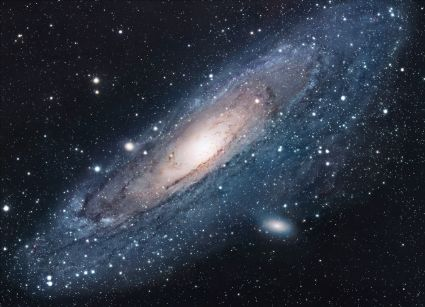
\includegraphics[scale=1.7]{universe.jpg}
	\caption{The Universe}
	\label{fig:univerise}
\end{figure}

\bibliographystyle{plain}
\bibliography{ref}
\end{document}
